% \documentclass[dvipsnames]{book}
\documentclass[dvipsnames,letterpaper,12pt,titlepage,oneside,final]{book}
\usepackage[utf8]{inputenc}
\usepackage{graphicx}
\usepackage{xcolor}
\usepackage{amsmath,amssymb,amstext}
\usepackage{tikz, pgf}
\usepackage{longtable}
\newcommand{\note}[1]{\begin{quotation}\color{ForestGreen}\textbf{Note} \newline \large  #1  \end{quotation}}
 \newcommand{\die}[2]{\frac{\partial #1}{\partial #2}}
\title{Draft}

\begin{document}
% \maketitle
\tableofcontents
% \note{this is a note} 
\section{Introduction}
\label{Sec:Introduction}
%\ref{Sec:Introduction})


\note{This thesis examines the complex system consisting of  housing markets, institutional investment, production, and the wealth of households.}

\note{To explore this system, we build an agent based model of a housing market, integrated with a model of a production and employment. We then adapt analysis tools from the study of resilience to analyze the transitions between alternative regimes, or patterns of functioning, of the system. We apply  an emerging formulation of resilience as a systems property, and associated systems dynamics analysis techniques. A unique feature of this thesis is that we examine the wealth trajectories of individual households within a spatially explicit urban model.} % that includes both a housing market and a model of production and employment. 

In ``Order without Design,'' Bertaud makes the case that cities are primarily labour markets' because labour markets drive the productivity of cities. 
%the reason labour markets are important is because they really account for the productivity of cities
%Yet labour markets are not well integrated into urban models. 
%He argues further that economic analysis more generally has not been adequately integrated into the work of planners and so cities are often planned in ways that fail to take into account the underlying economics.
The literature makes it clear that there are strong and  pervasive agglomeration effects driving productivity growth in cities (CITE). %and population growth. (City population is observed to follow a power law distribution.) 
These agglomeration effects interact with the cost of transportation, speculative real estate investment, and the cost of housing. 

The notion that the labour force is on average more productive when there are more people around is pretty dramatic and is not part of the basic models of production or urbanization. Our starting point is that's the fundamental feature of cities. 
We integrate that dynamic within a model that brings together a model of a productive urban economy with agglomeration in an agent based land market model to explore the effect of financialized capital.\note{Maybe say "with ongoing financialization of land markets"? }
What does that do with financial capital and what does that do to distribution and that's not been explored.
\note{Replace with:?  The impact of financialization on the distribution of wealth has not been explored in urban models.  ?}
It's not enough to understand these forces individually.
%Existing models don't capture the feedbacks between financialized investment, housing markets, and labour markets. 
The future of cities and the productivity of human capital depends on how they interact to drive the growth of wealth and amenity in cities. 

%In this work, we model how land rent is captured by landowners and how that affects wealth creation and the development of the city, using an agent based model to simulate key elements of a housing market. 

%Housing market consists of these things, but this model adds an additional layer that is usually modelled separately: a growth model that models the growth or shrinking of the city. 
%Modelling a housing market, a production model, and speculative investment together lets you see the feedback and interaction and they way that they feed into each other. That feedback relationship create rich resilience dynamics within the modelled economy. 

%Integrating the classical and neoclassical  distributional stories, we are able to look at distributional effects and the way they feed back into productivity. The agent based spatially explicit model of distribution with both financialized capital, an agent based housing market, and a model of urban productivity makes it possible to look at how people are affected: who gets to live in the city, who contributes, and who benefits? (Need to el)
%who gets the rents/surplus what does that mean for the class structure, and ultimately the productivity of cities

% More compressed and technical
% We couple two simple, standard models. The first is a Cobb-Douglas production sector, the second a basic Alonzo style urban system with transportation costs. Coupling the two allows us to illustrate  in a simple way the endogenous distribution of wealth and to describe the endogenous development of a class system in an urban economy.  The model is constructed so that there is neither land rent nor capitalist exploitation in the rural economy. This simplification allows us to focus on the distribution of the social surplus generated by agglomeration economies. 

The next chapter provides the theoretical background for the model, looking the scaling of wealth, rent, production, and the city. 
It outlines the history of rent and distribution and brings together these two distributional stories in one model. \note{Land rent has been largely ignored in recent distributional analysis despite its centrality in urban models. (instead of  :Rent was lost from the distributional story."?} One contribution of this thesis is integrating these two distributional stories to provide a more nuanced analysis of the challenges of urbanization, the nature of social wealth and how rent interactions with competitive markets. %Classical economics
The following chapter introduces the model of production, connects it with the urban scaling literature and develops a simple formulation for use in studying the interaction between financialization and production in an urban agent based model.
%As in the standard circular city model the constraint on growth is provided by transportation costs, which limits the size of the commuter-shed and therefore the labour force at any wage.
%Individual firms have decreasing returns, but the presence of agglomeration economies external to firms but internal to the city gives the urban economy as a whole increasing returns to scale. Excess return for urban firms drive both firm expansion and firm entry. The result is continuous growth of the urban economy. % What are the regimes in which the economy grows or does not
The chapter after that introduces the agent based land market model with renters, buyers, financialized speculative buyers and a productive sector. 
%We integrate this with a housing market model ELABORATE, and do resilience analysis.
The following chapters examine resilience and distributional effects in the context of the model. % provides a resilience based analysis of the model. 
%We then look at the resilience effects with 3 interacting layers of hysteresis 1. the productive capacity of the city 2. speculative rent seeking investment and 3. built form, increasing density as city grows. 

We formulate a measure of systems functioning, map the boundaries of the basins of attraction in the model, given hysteresis, and explore the effects of different classes of interventions. %  for shaping the pattern of functioning in the model.. tenure etc.

We argue that there exist regimes in which housing tenure acts like a peristaltic pump, pumping wealth out of communities in both economic boom and bust cycles. There is also a distinct regime in which housing tenure plays a role in building local wealth that can act as a buffer against rises and falls in the larger economic system. Ultimately, we hope our work will provide a theoretical foundation for those %, like our partners at CMHC, 
developing policy for affordable housing that centre household wealth. 

% Also It contributes to one set of tools for analyzing agent based models that is suited to the study of social innovation
%There is a distinction between use value and investment value. There is an argument between people who argue for using prices as a mechanism to grow the housing supply and those who push for policy priority should be centring the use value so people can live the city. - the rights, the minimum standards. We argue instead that (price is useful, there is real value-- at the same time the wealth of the city is a social wealth created by those who come to the city - who subsidize those who extract)

\section{Chapter: Model}
\label{Sec:Model}
%MAIN VERSION HERE IN OVERLEAF UNTIL MOVED BACK

%We build a spatially explicit agent model where agents work in one location and have transportation costs to travel to work. 


This work integrates a model of production and labour into a standard spatial model of the city. 
In this chapter, we introduce an analytic model of production and a labour market in a stylized circular city. 
We develop a spatial model with a labour market and agglomeration effects consistent with the literature as our base model. 
% Extended appropriately, this basic model could be used for planning.
We take a step beyond integrating labour markets in a city, to studying the distributional effects: who gets the surplus, what does that mean for the class structure, and ultimately the productivity of cities? 
% In this section we introduce the production function, introduce the labour supply and the urban model, the source of the surplus, then we calculate profit, consider who gets the profit, and from there we draw our conclusions.. then we calculate the urban surplus, and consider who gets it. 
%In subsequent sections we relax assumptions and look at how the interaction between the production of social wealth in cities interacts with housing and the extraction of rent to drive patterns in a richer model with heterogenous agents interacting over space and time. 
In the next chapter we will integrate a version of this production model in a spatially explicit agent based model with financialized investment. 

This model has two parts, first a production function, modelling how urban regions generate wealth, and second a model of an urban housing market. 
In this section, we introduce the basic structure of the model and examine the effect of agglomeration, using a circular city model.  
\textbf{The model has a Solow-Swan style production model with agglomeration effects using a Cobb-Douglas production function that incorporates Jacobs-style labour-augmenting agglomeration economies 
%(Beaudry and Schiauerova 2009, Panne 2004, J. Jacobs 1969), 
in the way neoclassical growth theory incorporates labour-augmenting technical change.}
It then integrates the production function with an Alonso-style urban model of a city economy (Alonso 1964). 
It is a model of a productive economy since the centre is productive and demands labour.

% Alternative phrasing 
%We integrate a labour market into a spatial urban model, set up to explore rent, and implications for the distribution of wealth.
%This model has two parts, first a production function, modelling how urban regions generate wealth, and second a model of an urban housing market. In this section introduce the labour supply and the urban model, we model the production function, then we calculate profit, consider who gets the profit, and draw conclusions. % The work draws on the Alfonso/Von Thünen model of the concentric city and Dawn Parker and Filatova's work in agent based modelling of housing markets (see http://jasss.soc.surrey.ac.uk/12/1/3.html 2009).% We begin with a simple model of a circular city with urban agglomeration effects. In subsequent sections we will use an agent based model to relax assumptions to look at how the interaction between the production of social wealth in cities interacts with housing and the extraction of rent to drive patterns for individuals over space and time.

The result is a simple model in which marginal productivity determines the wage, the wage determines the size of the city, the size of the city determines the labour supply, and labour supply determines marginal productivity. 
The model is constructed so that there is neither land rent nor capitalist exploitation in the rural economy. 
This special case allows us to examine the distribution of the social surplus generated by agglomeration economies and the effect of financialization.

In the simplest model, the central place pays a uniform wage, $w$ to all employees, who have identical preferences and transportation costs. $w$ is an attribute of individual residents. Residents  purchase or rent equal quantities of land at differing locations $l$ for identical housing.  

There are transportation costs $T$ that depend on distance from the  central place, so land close to the central place is more attractive than land farther from the central place.  

The equilibrium concept is that a market with identical individuals with identical incomes and transportation costs will result in identical utilities. The result is that land rent must decline with distance from the central place to offset rising transportation cost. 

The size of the city is determined by population and lot size. Income and transportation costs will interact with lot size. The basic model can be initialized by matching the number of properties to the size of the population. 


\subsection{A Circular City}

%Call it a radial city?
Following the Alonzo model [], firms are located at the centre of a circular city, the central business district. Residents residents live, spread across the space, and can take jobs and commute to work.
%In the simplest version, firms concentrate at the city centre. Workers are spread over space and pay transportation costs to commute.

Firms produce goods to sell. They can produce more goods by hiring additional workers. 
There is an agglomeration effect, which means firms can also produce more goods by operating in a city with more people, because of the connections and interactions between people (CITE). 
The simple circular city can be extended to to produce other forms, including polycentric cities and hierarchies of cities at the cost of additional computational complexity. The simple case we examine will allows us to focus on the general, and neglected, distributional features of this class of models.

\subsection{Labour Supply}

%The wage  determines how far people can travel, since it pays for subsistence, that surplus can go to travel, so the higher the wage, the farther workers travel for work. \note{Maybe } 

Workers in the countryside receive a subsistence wage, $\psi$, which could come from work in the local community, living off the land, family support, social support, or something else. % cite other models with subsistence wage.

Firms pay a wage premium, $w$, over the subsistence wage to attract workers. 
When workers take a job, they give up the subsistence income and instead receive the wage from their employer. 
The total wage employers pay is thus the subsistence wage plus the urban wage premium  $\psi + w$.
Specifying the model in terms of a wage premium simplifies the link to the production side and the treatment of household choice.

The urban wage premium determines how far people can travel. The higher the wage, the farther workers travel for work. 
Workers will go to work if the wage premium is greater than the cost of travel, $\tau$ per unit distance. 
Wage and transportation cost therefor determine the radius of the circular city, which determines the size of the labour force which affects urban productivity.  The cost of travel is therefore an important variable in the development of urban productivity. 

%Living close to work has value to workers because it saves the cost of transportation. 
%We assume workers receive a subsistence wage, $\psi$, in the countryside, which could come from work in the local community, living off the land, family support, social support, or something else. % [MAYBE ADD This follows xyz's approach, and makes it possible to explore resident's choice to work]. 

%If the cost of transportation is $\tau$ per unit distance, then t
The farthest workers will travel to work is thus $\frac{w}{\tau}$, which defines the radius of the commuter shed. Thus a worker, located at a distance $d$ from work, paying as much as $w-\tau d$ in rent, would still choose to work, and the maximum distance that workers will commute is the radius of the commuter shed. Given a uniform lot size $s$, with one worker per unit land, the labour available is the area of the city. In the circular city, this is the area of the circle divided by the lot size
\begin{equation}
                 L%=  \frac{\pi}{s}(c^{max})^2	
			=\frac{\pi}{s}  \left(\frac{w}{\tau}\right)^2
			=\frac{\pi}{\tau^2 s} w^2, \label{Eqn:LabourSupply}
\end{equation}
which increases with the square of the wage. This is the equilibrium urban labour supply curve.

As in the standard circular city model the constraint on city size and hence growth is provided by transportation costs, which limit the size of the labour force at any wage. 
% Rising transportation costs can become the limit on firm or city expansion. 

%To get wage, we can write thee  inverse labour supply function  is
%\begin{equation}
%	w= (\frac{ \tau^2s}{\pi})^{0.5} L^{0.5},	%\label{Eqn:InverseLabourSupply}
%\end{equation}

 % TODO:  FOOTNOTE the transportation cost/distance relationship appears to be non-linear in many cases. While the linear model connects with the established literature, we likely want to explore the implications of more empirically grounded curve (e.g. Alain Bertaud, 2015)
% More generally, if we were to introduce variations in lot size and housing types  we would want the integral of the worker density function. In our ABM version  of the model we simply count the workers within the commuter shed.

% DETAILS AND ALTERNATIVE PHRASING  
% MARGINAL PRODUCT The marginal product of labour is monotonically declining, ensuring a labour market equilibrium, to connect with the analytic tradition of economic modelling by ensuring there is an equilibrium level of production.  While adding more labour may always adds some value, the rate at which it adds value drops off. 
% If the marginal product increased, then a firm that got large enough would out compete smaller firms, hire all labour, always be able to produce more wealth by hiring more people, and would always produce more wealth by hiring people than by firing people. This doesn't happen. 
% Perhaps, the firm hires employees who best fit its needs first, but to grow, eventually it must hire less selectively. Finding markets may get harder with growth. Perhaps expansion adds additional costs, building a parking lot, administration, acquiring a larger building. Whatever the explanation, the marginal product of labour declines. 

% Frictional unemployment usually just refers to people moving between jobs. When people look for jobs, it may take time to get them. The analytic model offers an equilibrium solution with full employment. In the agent based model this assumption does not hold, workers are laid off, and take time to find new employment.
% labour adjustment costs include moving costs for the employee or hiring, firing, or training cost for the firm. (there might be a hiring, firing, or training cost on the firm side, or on the employee side: expected time to employment costs, moving costs, etc.)
% The assumption of monotonically embedded marginal product of labour is embedded in the production function, so it applies in the analytic and agent models. This appears in the requirement that the sum of the exponents in the Cobb Douglass are less than one without agglomeration effects. Agglomeration effects can push the sum above one. When the exponents add up to less than one, there are diminishing returns to scale.  Exploring alternatives would involved exploring other formulations of the production function.

% $mvp(x) = p(x)$ where x can be labour, capital or any other factor, falls out of the function when you introduce profit maximization. Continuity and differentiability assumed but it is a convenient approximation-- take away assumptions you typically get a close approximation.

%We have a two factor model of production with labour and capital.  


\subsection{Production}

Firms produce goods which they sell in a commodity market\footnote{For simplicity, assume firms produce a variety of perfectly substitutable commodities which are exported and locally consumed at a fixed price in a large market. Note increasing product variety may produce a consumption agglomeration economies as in \cite{FujitaKrugmanVenables}.}. Demand for the urban product is perfectly elastic which means producing more won't affect the product's price; and there are decreasing returns to scale, which means each new worker increases output by less than the last worker did. 
  
We use a two factor model of production, where production, is a function of capital and labour. The firm maximizes profit by setting the marginal value of the product of each factor equal to the unit cost per factor. We model agglomeration with a Solow-Swan style term for labour augmenting technical change. In the Solow-Swan model 

 \begin{equation} 
Y(t)=K(t)^{\alpha }(A(t)L(t))^{\beta }
\label{Eqn:Solow-Swann}
 \end{equation}
where $Y$, $K$ and $L$ are aggregate output, capital, and labour, respectively,  $A$ is the term the Solow-Swan model introduced for technology, that can capture the growth of labour productivity over time, $\alpha$ is the elasticity of output with respect to capital, $\beta$ the elasticity of output with respect to effective labour, and $t$ time. If $\beta=1-\alpha$, this is a constant returns to scale (CRS) production function at the firm level.

% In the Solow-Swan model all factors of production are fully employed, and initial values $A ( 0 )$, $K(0)$, and $n( 0 )$  are given. The number of workers, i.e. labor, as well as the  level of technology grows exogenously at rate %s are $n$ and it   $g$,% respectively:     $L(t)=L(0)e^{nt}$     $A(t)=A(0)e^{gn}$ 
 
This model uses a similar functional form to look at  the effect of population density increasing % productivity. %how density increases in in  % It models how population increases productivity. $\Lambda(n)n$ is  ``effective labor'' 
 the productivity of labour, rather than technology growing productivity over time. With labour augmenting agglomeration, $\Lambda(n)$, in place of technology, the equation becomes 

\begin{equation} 
Y=K_i^{\alpha }(\Lambda(n)n_i)^{\beta }.
\label{Eqn:Prod1}
\end{equation} 
where $n_i$ is the number of workers at the firm, the labour, and $n$ is the urban population. The agglomeration factor increases with population. It multiplies labour because agglomeration scales the productivity of workers. 

A natural functional form of the agglomeration effect for illustrative purposes n is $\Lambda(n) = n^\gamma$. Then:

\begin{eqnarray}
 Y&=K^{\alpha }(n^{\gamma}n)^{\beta}  \nonumber\\
 Y&=K^{\alpha }n^{\beta(1 + \gamma)}.
 \label{Eqn:Prod2}
\end{eqnarray}
If $\gamma=0$ there are not agglomeration effects. Notice that  this formulation implies it is possible to have increasing returns to scale for the urban economy even with a production function at the firm level with decreasing returns to scale: the return to the total economy $\alpha + \beta(1 + \gamma)$ can be greater than one, even if $\alpha +\beta$ is less than one. %.\label{Fn:PSI}}  
(CITE Appendix: Excess Returns)

Assume $\Lambda(1)=1$ so the agglomeration effect has no influence with one person in a multiplicative function like the Cobb-Douglas, and %$\die
FIX die ${\Lambda}{n}>0$, so it is increasing with population.

%%%%%%%%%. ***WHY
If $\beta=1-\alpha$, this is a constant returns to scale (CRS) production function. Without agglomeration effects, $T(n)=1$,  Then  \textbf{$\mathbf{L(n) = T(n) n}$} 

% Without agglomeration effects, $\Lambda(n)=1$,  Then  \textbf{$\mathbf{L(n) = T(n) n}$} }

% Firms will purchase the time of workers to capture the product of their effective labour % and enjoy the product of effective labour. %was If labour markets are competitive, it will set 
%$\die{Y}{L}=w$.
%*** DEFINE EFFECTIVE LABOUR, COMPETITIVE MARKET
% Effective labour is the productive output from labour. As soon as you introduce agglomeration economies, labour becomes a more complex phenomena. There is the benefit of the single worker which should be perfectly declining on that nice concave production function and there is the diagonal movement as a result of increasing productivity because you keep adding people to the market. That means that your productivity of the worker isn't' just attached to the worker and your plant. It has this other component.. 'effective labour' -- the output including the A term.
% Labour always depends on the human capacity, technology, tasks aside so it is always complicated
%Capital is always complicated too it has dates, whether you can get the inputs for it, whether they're produced nearby etc.. -- 

%** ``The notion that your labour force is on average more productive when there are more people around is pretty dramatic and it's very much not part of the basic model that we use. Our starting point is that's the fundamental feature of cities, and what does that do with financial capital and what does that do to distribution and that's not been explored.

%Competitive market- everybody is a price taker they don't assume.
%price takers don't assume anything you do affects other producers or suppliers .. so you act in terms of account your internal prices and costs.
%Take into account any one else's behaviour
%the easy way to see that is assume prices are fixed - all that's required to get the behaviour.

%* have a few other things like free exit and entry, perfect information etc -- to get the efficiency result. - (or to ensure price taking)

%Monopolists knows that increasing output will require a reduction in price-- and take into account how consumers will apply and take it into account.
%No externalities imperfect information etc.. ensure efficiency but aren't needed, all you need is price taking for individuals to only pay attention to their own costs and their own benefits. 

%competitive markets many sellers, many buyers, monopoly single seller, monopsony - single buyer, intermediate cases - monopolistic competition - with some market power but not complete - duopoly- some inefficiency depending on the behavioural model because in the duopoly case they may be able to take advantage of the behaviour of buyers.
% Start with perfect competition, then introduce monopolistic competition is most likely.. but it's more difficult to handle. e.g. with brand names, people have some preference for some feature of your particular good so you can price it higher even though you may loose some marginal people. Firms compete on brand name and reputation, not the pure cost effect.
% In the spatial economy, goods are deferentially interchangeable. Put them on a line and firms pick a place along they line. Firms are in competition but are competing on a line-.. spatial model moved over to characteristic space.. -- looking at this would involve overlaying another space - the characteristic space on the physical space. .. There are also local places with local grocery stores. Polycentric stores have effectively monopolistic competition in real space. - like a named cafe downtown has the same.
% Market power means you can price above marginal costs. Need free entry to get rid of it. -- it doesn't drive out profit - profits can be sustained over longer.
% Monopolist can charge a higher price but pays competitive price for all inputs including labour. If a firm also had a monopoly on offering jobs, they could drive down wages.

%Firms calculate what the next worker is worth to them. That's what they're willing to pay for labour. 
%This is the labour demand function based on the marginal product which is declining. When a firm has only a few workers, it is high on that demand function, and has to move down. It cuts workers. If it's too low, it expands and hires. Note this says something about the geometry of what employers could pay. Firms can't pay workers more than they can earn in the long term, unless that money comes from somewhere, but they could push down wages and extract more profit, invest more in other factors of production, etc

To maximize profit 
% firms set the marginal value product of labour, $p\die{Y_i}{n_i}$, equal to the wage. 
in a competitive market, firms offer a wage equal to marginal value of labour, 
%$p\die
FIX p die ${Y_i}{n_i}$, where $i$ indicates the $i^{th}$ firm. In the analytic model, there is no frictional unemployment, there are no labour adjustment costs.\footnote{Note: we do not assume equilibrium conditions in the agent model, however our approach is to stay close to the analytic tradition, relaxing assumptions to clarify what drives each results, and connect the work with classical and neo-classical theory.}. % For instance in the agent model, employees are simply laid off and seek work, so there is unemployment, but there are not labour adjustment costs for firms.}. For convenience, price per unit is one. 

A labour market equilibrium exists if the marginal product of labour, is monotonically declining, which it is with a Cobb Douglas production function, and $\alpha + \beta<1$ 
Population would be expected to adjust much more slowly than firm wages, so labour supply should converge. The case where there are increasing returns at the city level introduces interesting dynamics, explored in appendix CITE % 'furthur discussion' appendix.

%To ensure there is a labour market equilibrium to study in the analytic model, the marginal product of labour declines monotonically, 
%***ILLUSTRATE AND CLARIFY
%If you see it as just supply and demand .. 
%Supply demand with fixed product and everything’s neat
%Agglomeration changes everything,.. firms are underestimating each time they add a worker, the value that’s going to be produced. They benefit from an agglomeration effect and that’s where they interesting dynamics are coming from..
% we know that there is a marginal product of labour for a firm that it should be able to figure it out.. can the person on the shop floor figure out whether it's worth hiring another person.. we can talk about it, add details etc. We have a declining marginal product of labour. Because of transportation costs, we have a rising cost of getting labour so they cross and there is an equilibrium. There are adjustment questions like which adjusts quickly, how fast people move in, how fast firms decide to hire etc, but we know that there is in principle and equilibrium and that it is in principle a stable equilibrium (DIAGRAM STROGATS) although there are complications with this-- some argue these market equilibria never make sense- true in lots of way, but useful for analysis. 
% The question is then, what happens in our city? Do you get a growth dynamic? What seems to be the case is that if all the firms add workers then the marginal value of the product of all the workers they have goes up, which means they are making more profit which means if they are making more profit they want to hire more workers? Does it ever converge? Likely eventually, but it's got a very powerful dynamic.  If you add other features like more products being created in the city, which is part of this agglomeration process you can start seeing, if you exhaust one source of growth, we know that there are others, that simplification is just firms of the same sort hiring workers of the same sort is wrong. so we need to add the local service sector, we need to add the possibility of creating new products and those depends on the number of workers and so depend on further agglomeration effects. What does this mean? For the purpose of the model, we'd want to strengthen the agglomeration effect relative to what they are for specific firms or industries..

Population/workforce, $n$, and the wage will be determined endogenously in competitive markets. 


 \subsection{Rent}
\label{Sec:Rent}

%``We model how land rent is captured by landowners and how that affects wealth creation and the development of the city. 

%Land is a monopoly good \note{talk about what you mean by monopoly good?} 
The supply of land at any distance from the center is inelastic. 
Its value comes from proximity to the productive urban centre, not from the value of improvements made to the property. 
% Reference sections on development which is different, and the contribution of amenity % Because supply is fixed for urban land, and the landowner has a monopoly claim on rents, the rents that can be depend on wages and amenity rather than the cost of improvements made to the property.
% The source of rents is the free gifts of nature, the coming together of people to create value in cities, and the concentration of public amenity in cities. 
In the circular city with linear transportation costs, the maximum rent for living closer to work is at distance $r$, from the center, is $w-\tau r$.  is Workers could pay that much and it would still be worthwhile to commute to work. 

Rents go to landowners. %the owners of a given property. 
Landowners therefore capture a fraction of the wage premium generated by agglomeration.

If workers own their own homes, rents go to them. If others own the land, they capture them. %\note{REPHRASE? rent is  extracted from the coalition of capital and workers.} % Rents may also be taxed, could be shared between multiple owners, etc. 
%The rents are captured by landowners.  The capture of rents by landowners is common buy not necessary. 
In principle the gains from urban productivity and amenity can be allocated as social wealth through shared ownership, as is often done on a small scale with cooperatives and land trusts, distributed to all citizens through something like a social wealth fund, or captured in taxes or fees as Henry George suggested. 
%The rents would otherwise go to labour and capital.

% Agglomeration benefits get extracted by landowners. Labour gets only their marginal value they don't get any of the surplus. They don't even keep always their marginal value.
the dynamic story is that the class of landowners eventually becomes financial capital.
PLOT RENTS HERE

The value of land increases over time. Those who purchase land earlier claim a share of the growing value of the city. % As the city grows, they own an increasingly valuable asset.
 
%In this model, workers are the initial owners, but they build this wealth which becomes a source of capital that can support them.

EQUATION FOR THE SHARE THEY CAN CAPTURE


\subsection{Demographics}

Workers can leave the workforce and retire, and new people can come into the city. Land value rise as the city grows, so newcomers pay more for housing near the centre.

In the case in which individual workers purchase houses and then sell them on retirement, the housing market drives the creation of classes on its own. A strictly random process in which agents have a range of ages and sell at retirement creates a structural advantage where workers who arrive earlier in the city and own land, benefit from their own labour but also get to claim a share fo the productive output of the city as it grows. % those who begin work later. % to a division in wealth
%the emergence of a class of those who came early and those who came late.
%Early agents may also rent out their land. Could it be though of as a pyramid scheme?

In the classical language, someone is exploited if someone else gets a share of the value of their labour. %(REPLACE WITH MORE PRECISE DESCRIPTION). 
 Employers capture a share of the value of workers' labour, so they exploit workers under this definition.
Those who own land early in a growing city are also capture a share of everybody's production. Since they capture a share of the productivity of others working in the city, through the rents, they are also exploiters, they form a kind of hybrid class. %Rents could be captured directly through renting out the property after they retire away from the city,  or by selling the property at a higher value than they bought it. 

% MARGINALIST DISTRIBUTION
%we've been paying some people less than the market wage so our profits our higher. this is what it would be if we paid everybody
% FOOTNOTE - RELATIONSHIP with marginalist distribution story ******** TODO Does the marginalist approach assume they are not exploited? Is it an experiment in examining the case where production is non-exploitative? 
% In a sense if labour gets the marginal value of their product, are they exploited. It's a matter of interpretation.  -It has an attraction 
%Clark tried to make an ethic of this. if everyone is being paid the marginal product of their labour. We know that's an efficient outcome. If it's efficient, is it also fair
%Is it possible someone's taking out an extra large fair. Yes. Not fair for simple classical reason that labour has been exploited in the past and that the current owner ship is a result of exploitation. The ownership of land introduces a kind of exploitation-- clearly exploitation if you claim that. 
%Lot's of marxists didn't like Henry George making it a locational question, they wanted to keep it located in the factory.
% You could - well what value did they create -- in line with those other-- could interpret.. 
%What is the average value, because every worker is not just marginal, they're also average/identical. What is the value created by the whole of the workforce. Should they be paid the marginal value or the average value of their work.
%
%The avg value -- declining.. 
%The demand for labour is declining--  
%Every infra marginal worker has been paid less than the avg contribution 
%Every infra marginal workers should - 
%every marginal worker should get the average wage.. that's fair.
%
%Get to the margin - that's what you pay.. that's what the next worker is worth to the firm. .. 5th' worker is paid more than the 10th. should it be averaged out and paid to all workers? paid to worker, or should the difference between top and the marginal goes to the firm- -- that's profit.. pay everyone the marginal value and keep the rest as profit.. 
%Effective labour has a higher marginal product.. - even higher - higher for the firm.. - but they don't have to pay the workers that... firms only have to pay enough to get their marginal individual cost down to the wage. The problem there is if they're making more profit they want to expand the workforce, but that wage only supports a certain size of city -- they've got off raise the wage a bit.. so they face an upward sloping supply curve for labour=-- that's why you know there's an equilibrium.. declining product and upward sloping supply so they cross.
%
%(all the profit you earn on the way could be redistributed)

\section{Chapter: Land Market}

Urban productivity %and amenity
drives land values through the housing market.%Agents purchase homes to live in. The value of the the proximity to work and to amenity drives shapes the what agents are willing to pay. 
% These prices shape the relationship between housing markets and the wealth of households.
Our goal is to look at the relationship between housing markets, financialized investment, and production. % and labour markets. 
To explore this relationship, we integrate the model of production developed above with a spatially explicit agent based land market. % in which heterogenous individuals and institutions buy and sell properties given their individual goals, resources and available information. We integrate this housing market with % within this model of individual and institutional actors in a spatially explicit property market, a model of production and employment.

We examine the effect of housing on wealth inequality by looking at 
%We explore the wealth forming dynamics of the urban agglomeration effect by modelling 
a city in which agents work in the city and leave their jobs when they reach retirement age. They may choose to rent or sell their home. %?They may chose whether to stay in the city, if there is sufficient amenity value for them, to rent their house, or to sell it. % Todo can agents choose not to retire? Can they keep working? Do they get the subsistence wage on retirement? Do they need to leave the city to get it? 
New agents enter the city to work. 
Agents fund their retirement from savings, as well as returns on their home if they own one. Savings may be invested in a pension fund, or in local property,  depending on expected risks and returns. % either in the stock market, or in pensions.
A financial institution manages the pension, investing in the market or in property.
%Institutional and individual investors can access debt. %We also consider a case where outside money can come under institutional management, not just local retirement savings. A parameter controls the inflow of additional money beyond local investment in the pension fund. 

% There is an outside world in two respects. There is a market for the urban product produced by firms, and a financial market that agents can invest in.
% Lots of simple extensions e.g. 2 cities with immigration, differentiated labour, products, market power, neighbourhood effects (see extensions map/typology), we focus on those elements central to seeing the structure of the resilience dynamics of the wealth/housing effect. Consider adding density, to look at how it interacts with agglomeration effects. (integrating with transportation effects is very neat)
 
 If there is a housing market, agents can move. %In the analytic case above, the population stays in place, and travels to work if it is worthwhile given the transportation costs. 
%Those who come to the city will be those for whom the benefits the city offers make it worthwhile to  whether that's building their network, accessing markets, accessing amenity, learning, finding specialized employment, or increased wages. In this model 
The demand for labour drives urban growth. % The housing market depends on how many people from the periphery are completing to claim places in the city. TODO IF ANY RURAL AGENT COULD MOVE IF THE CITY HAS ADDITIONAL DEMAND FOR LABOUR, HOW DO WE DECIDE WHICH DO? Could use a parameter for immigration (or how 'hot' the market is) and in the simplest case (corresponding to how many agents from outside are looking at the housing/rental market), have the inflow match. % Agents have debt and there is an undifferentiated labour market
 % We may. 
 
Figure xyz traces the flow. In each time step agents firms update wages and job availability, agents decide whether to work and whether to buy and sell homes.
 % Schedule: Multi step by breed
 % Steps Labour
 % step - workers: market/production, enter market to buy, list properties real estate agent matches agents - has bids 
 % bidding - workers and firm consider properties and make bids (2nd step or spread over 2 steps)
 % negotiation - sellers consider and accept bids (or real estate agents manage negotiation)
%Buyers evaluate their need for housing.
% Agents decide whether to enter the housing market as a renter or a buyer.


 
Worker agents from outside the city can always consider moving and accepting a job. % QUESTION - how to manage the flow of new agents?
%, or can make more from rents and moving away (with a non-differentiated workforce)
% They need to approximate housing prices to know if it makes sense to work. Do they use past prices?
% 
% 
The higher their need, the more houses an agent considers, and the more willing they are to negotiate on price. % Buyers rank their housing need on a scale of one to ten. 
% Maybe later: Buyers could consider neighbourhood pressures, demographic changes, changes in job location, desire for amenity etc. in their assessment of housing need. 
Buyers then consult with a financial agent to determine the maximum mortgage and interest rate they'd qualify for based on their income. This gives an upper bound to the range of homes they may consider. 

Next buyers request a selection of homes to consider from a real estate agent. Those with higher need for housing look at more homes. The real estate agent offers a selection of homes based on the agent's requirements. A randomness parameter determines how many divergent houses are also considered. When the parameter is 1, the selection of homes is fully randomized, When it is 0, the agent sorts all available homes and offers those which fit the agents budget, space, and other requirements best.

Finally agents rank all the homes offered and place bids.  For simplicity of implementation, they place bids on all homes they consider. They place the most competitive bids on those homes they prefer. If they have higher urgency they place strong bids on more homes. 
A utility function/algorithm specifies agents preferences over the attributes that matter. - algorithmic continuous. lexographic- any traits. 

Finally Variables from last time also affect desire and urgency in the next time step. If there is a good fit/price ratio, their assessment of desire increases. If they dislike what they see, their desire decreases -- they settle for what is there. 



%Calculate willingness to pay
%Consider options
%Place bids
%
%Calculate willingness to pay (urgency/position on the market)
%Assess need for housing
%- Urgency of need Unhoused, sold house or served notice? 
%- Family or demographic changes
%- Financial viability of current situation
%Assess financial situation
%Get Max mortgage and max carrying cost given income and wealth from a bank
%Get options from real estate agent
%Place bids based on xy
%Consider options
%Place bids
%
%
%
%BUYER
%
%Enter market to buy
%Decide level of urgency (or decide with prospect theory - functional form for optimism/urgency/time to choose)
%(income/wealth)
%Maximum mortgage 
%Maximum carrying cost
%Household attributes - household size, employment location, amenity
%Current housing
%
%Realtor gives list of houses to look (real estate search -e.g. price range)
%Place offers - low if can't afford, higher if market is tight
%If failed, consider renting or buying next time.


 \tikzstyle{decision} = [diamond, draw, fill=blue!20, 
     text width=4.5em, text badly centered, node distance=3cm, inner sep=0pt]
 \tikzstyle{block} = [rectangle, draw, fill=blue!20, 
     text width=5em, text centered, rounded corners, minimum height=4em]
 \tikzstyle{line} = [draw, -latex']
 \tikzstyle{cloud} = [draw, ellipse,fill=red!20, node distance=3cm,
     minimum height=2em]
%
 \begin{center}
 \begin{tikzpicture}[node distance = 2cm, auto]
     % Place nodes
     \node [block] (need) {Assess need for housing};
     \node [block, below of=need] (finance) {Assess financial situation};
     \node [block, below of=finance] (alternatives) {Select homes to consider};    
     \node [block, below of=alternatives] (bid) {Place bids on homes};    
     % Draw edges
     \path [line] (need) -- (finance);
     \path [line] (finance) -- (alternatives);
     \path [line] (alternatives) -- (bid);        
 \end{tikzpicture}   
 \end{center}




\subsubsection{Financialized Capital}

%Individuals and institutions play a role in the housing market through credit markets and direct investment.Agent's access credit shapes worker's ability to purchase homes. Credit is offered by institutions.
% Agents may be able to foresee future growth. %They may even over invest if they follow market trends and bubbles form. 
% They can claim a share of the urban wealth as it grows over time by owning the land. 

If the return on housing investments is competitive with alternative investments, capital from institutions and individuals will flow into housing. Institutional investors can purchase housing.  Individual households can also allocate a larger share to housing to capture the returns.
% If the return on investment in housing is competitive with alternative investments, can purchase housing for it's financial return. They can rent housing and sell the asset with appreciation later. We examine the conditions in which this increased demand can drive up prices in the market. 
% Capturing future growth of the city, depending on their foresight - how much does it take to block individuals from gains-- Regime.
% both institutional investors and individual agents can purchase additional housing for it it's return on investment even though they don't need it as a place to live. 
% Use value vs rent value. 
%Institutional investors can purchase housing as an investment. Individuals with more wealth may invest 
Households may, for example purchase a larger house than they need, purchasing additional units to rent out, or keep a house after retiring rather than downsizing.  % and individuals with sufficient means can purchase larger homes than they need to benefit from appreciation, or purchase additional units to rent to others. 
% Investors can also purchase housing to claim a share of the future productivity of the city. Individuals and groups can put extra money into housing. Institutional housing providers can buy up the housing supply.
% HYPOTHESIS FEEDBACK LOOP -- FINANCIALIZED INVESTMENT --
%The rise in spending on housing as a proportion of income can be driven by both rising prices (cutting into quality of life) and increasing investment to claim a share of the returns.  -- disaggregate and show the geometry -
% Test how linear is this relationship? 

%With financialization, in the case where 
If financialized buyers can access a better interest rate, they can consolidate ownership, capture rents, drive class differentials, and amplify wealth inequality. % This appears to be the case as lenders offer wealthier and larger entities lower interest rates. % We expect to observe in this class of models larger, likely power law-distributed, wealth effects.

%There is a supply of money- if there's too much for other investments, some will flow here- e.g. excess liquidity.



\subsubsection{Size of mortgage available, $m_i$}
\[m_i= \frac{0.25Y_i}{r_i}\]
where $r_i$ is $i$'s cost of capital, $Y_i$ is $i$'s income.

\subsubsection{Cost of capital $r_i$}
The cost of capital is known to differ for rich and poor. Say for example, the cost of borrowing, $r_i$ for agent $i$ if the base lending rate is $\bar{r}$
 \[ r_i = (A + B \frac{\bar{W}}{W_i})\bar r\]
where $\bar{W}$ is mean wealth and $W_i$ is individual wealth. %Figure~\ref{Fig:BorrowingCost} illustrates the effect.

%\begin{figure}[htb]
%\begin{center}
%\chapter{SAPriceOfCapital}

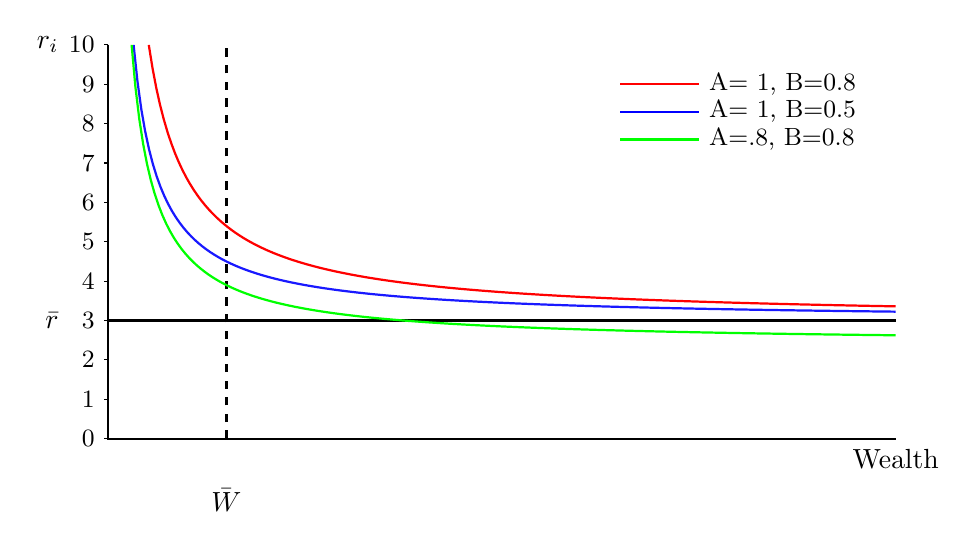
\begin{tikzpicture}[scale=.5]
%\def\bndmax{5}        %https://tex.stackexchange.com/questions/68462/filling-a-complex-region-with-tikz
%\def\bndmin{0.2}
\def \Y {10}  % height of y axis pecent
\def \W {20}  % length  of x axis
\def \Wbar {3} % jmeam wealth
\def \omega {3}
\def \A {1}  %was .5
\def \B {.5}
%Equation   \[ r_i = (A + .5 \frac{\bar{W}}{W_i})\omega\]
\def \Wmin{.63}  %This sets the lower limit fo the 
\def \Wmin{(\B*\Wbar)/(\Y/\omega-\A)} %function to keep in in bounds
	
\tikzset{func/.style={thick,color=blue!90}}	

\draw [thick] (0,\Y)node[left=.5cm]{$r_i$} -- (0,0)--(\W,0)node[below]{Wealth};  	% Axes
\draw [thick] (0,\omega)node[left=.5cm]{$\bar r$} -- (\W,\omega);  	% Axes
\draw [thick,dashed] ( \Wbar,0)node[below=.5cm]{$\bar{W}$} -- (\Wbar,\Y);  	% Axes

\foreach \yi in {0,...,\Y} \draw (0,\yi)--(-.1,\yi)node[left]{\small$\yi$};

\draw[func,domain=\Wmin:\W] plot [samples=200] (\x,{(\A+\B*\Wbar/\x)*\omega});
\def \A {.8}
\draw[func,domain=\Wmin:\W, green] plot [samples=200] (\x,{(\A+\B*\Wbar/\x)*\omega});

\def \A {1}
\def \B {.8}
\draw[func,domain=\Wmin:\W, red] plot [samples=200] (\x,{(\A+\B*\Wbar/\x)*\omega});

\draw [red,  thick](13, 9)--(15,9)node [right, black] {\small A=\ 1,\ B=0.8};
\draw [blue,  thick](13, 8.3)--(15,8.3)node [right, black] {\small A=\ 1,\ B=0.5};
\draw [green, thick](13, 7.6)--(15,7.6)node [right, black] {\small A=.8, B=0.8};
 \end{tikzpicture}
% Figure of cost of borrowing
%\caption{Hypothetical wealth-dependent borrowing cost}
%\label{Fig:BorrowingCost}
%\end{center}
%\end{figure}%

This has a number of immediate implications. First, if agents discount at their borrowing rate, wealthier agents a lower discount rate and therefore value properties more highly. 

Second, given the  common rule that mortgage payments cannot exceed some fraction of disposable income, the wealthy will be able borrow larger amounts and at lower interest rates that the less wealthy. At any distance from the centre they will be able to make a higher bid.
 
If the expected return on a property is greater than the individual cost of borrowing, it would pay any agent to borrow as much as possible and purchase properties as they become available.

\subsubsection{The rate of return on a property purchase $v$}
To explore the implication of the financialization of the urban land market we need a function to calculate the return on a unit of land that reflects the actual gradient of opportunity in financial markets. We begin with the price appreciation, $\Delta P=P_T-P_0 = (1+\dot p)P_0-P_0 $, where $\dot p$ is the rate of price appreciation over the period $T$. Rates will all be specified for the period $T$. Transaction costs, including real estate fees, take a fraction from the value of the final sale.

 The speculator invests a down payment, $D$, and gets back at time $T$ the  increased price $(1+\dot p)P_0$, plus rents, minus any costs and minus the mortgage with interest.
%footnote{We can include a use value, $U$ in place of rent for expatriate owners to represent using the property - say one month a year - when they are not renting the property and a \textbf{vacancy tax},
%$T$ at rate $t$ to affect the speculator's  decision.
 
The rate of return is the value of the gain, $V$,  over the size of the downpayment, $D$, where
\begin{equation}
V =capital\ gain - Interest\ due  	+ Rent  - operating\ cost\    
\end{equation}

The rate of return is $v = \frac{V}{D}$. 

Both the  share of the price  that can be mortgaged, $m$, and the interest rate  and $r$ may be functions of the agent's wealth. $\delta$ represents the net capital gains tax. It makes it possible to capture the capital gains kept. If it is set to one, it simplifies the equations, all is kept. Keeping the variable offers a policy variable to control the return on financial capital.

\begin{eqnarray*}
V  %	&=& capital\ gain - Interest\ due  	+ Rent  - operating\ cost\\
% 	&=& \delta P_T-D \qquad \qquad \quad - (1+\delta r)M \quad	 + R  	-C\\
% 	&=& \delta P _T \qquad-(P_0-M) \quad- (1+\delta r)M 	 + R  	-C\\
%	&=& \delta (1+\dot p)  P_0 -(P_O -M)  -(1+\delta r)mP_0  + R  -C\\
%	&=& \delta (1+\dot p)  P_0 -P_O + M \qquad -(1+\delta r)mP_0  + R -C\\
%	&=&( \delta (1+\dot p)-1)  P_0  + mP_0 \quad -(1+ \delta r)mP_0  + (\rho-\kappa)P_0\\	
%	&=& \left(  \delta (1+\dot p)-1    + m \quad - m(1+\delta r)  + (\rho-\kappa)\right)P_0\\'
%	&=& \left(  \delta (1+\dot p)-1    + m \quad - m-\delta rm  + (\rho-\kappa)\right)P_0\\
&=& \delta(P_T- (1+r)M) \qquad \qquad 	 + R  	-C   - T\\
&=& \delta((1+\dot p)  P_0- (1+r)mP_0)   + \rho P_0  	-\kappa P_0 - tP_0\\
&=&( \delta((1+\dot p)  - (1+r)m) \ + \rho   	-\kappa -t) P_0
\end{eqnarray*}

This is the  net present value of buying, and selling after one period. \textbf{It has  6 exogenous parameters}. Operating revenue and costs $ \rho -\kappa - t$ a present value. 

The rate of return is $v = \frac{V}{D}$. For expat investors, we get a \textbf{decision rule}:\begin{enumerate}
\item  if $v \geq a$ (with some private use?) with no rent,  don't bother renting. 
\item If $v(no\ rent\ and\ tax) < a\leq v(with\ rent)$,  then  rent. 
\item If $ v(with\ rent) \le a $,  then sell 
\end{enumerate}


We can, with some simplifications, write
\begin{eqnarray}
\frac{V}{D}&=&( \delta((1+\dot p)  - (1+r)m) \ + \rho   	-\kappa - t ) \frac{P_0}{D}   \nonumber\\
		&=&( \delta((1+\dot p)  - (1+r)m) \ + \rho   	-\kappa - t ) \frac{P_0}{P_0-mP_0}   \nonumber\\
		&=&\frac{ \delta(1+\dot p  - (1+r)m) \ + \rho   	-\kappa - t } {1-m} \label{Eqn:DecisionRule}
\end{eqnarray}

\subsubsection{Returns on capital are higher for wealthy investors}
\[   r^h=\frac{ \delta(1+\dot p  - (1+r)m) \ + \rho   	-\kappa - t } {1-m}    \]
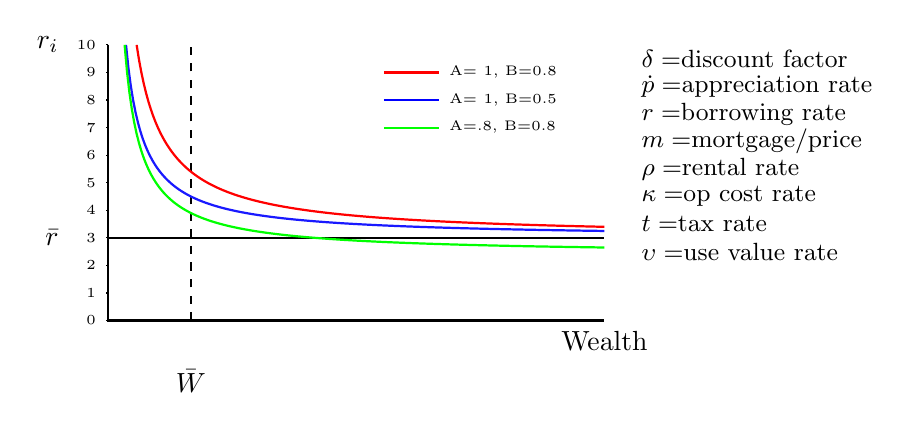
\begin{tikzpicture}[scale=.35]
%\def\bndmax{5}        %https://tex.stackexchange.com/questions/68462/filling-a-complex-region-with-tikz
%\def\bndmin{0.2}
\def \Y {10}  % height of y axis percent
\def \W {18}  % length  of x axis
\def \Wbar {3} % j mean wealth
\def \omega {3}
\def \A {1}  %was .5
\def \B {.5}
%Equation   \[ r_i = (A + .5 \frac{\bar{W}}{W_i})\omega\]
\def \Wmin{.63}  %This sets the lower limit fo the 
\def \Wmin{(\B*\Wbar)/(\Y/\omega-\A)} %function to keep in in bounds
	
\tikzset{func/.style={thick,color=blue!90}}	

\draw [thick] (0,\Y)node[left=.5cm]{$r_i$} -- (0,0)--(\W,0)node[below]{Wealth};  	% Axes
\draw [thick] (0,\omega)node[left=.5cm]{$\bar r$} -- (\W,\omega);  	% Axes
\draw [thick,dashed] ( \Wbar,0)node[below=.5cm]{$\bar{W}$} -- (\Wbar,\Y);  	% Axes

\foreach \yi in {0,...,\Y} \draw (0,\yi)--(-.1,\yi)node[left]{\tiny$\yi$};

\draw[func,domain=\Wmin:\W] plot [samples=200] (\x,{(\A+\B*\Wbar/\x)*\omega});
\def \A {.8}
\draw[func,domain=\Wmin:\W, green] plot [samples=200] (\x,{(\A+\B*\Wbar/\x)*\omega});

\def \A {1}
\def \B {.8}
\draw[func,domain=\Wmin:\W, red] plot [samples=200] (\x,{(\A+\B*\Wbar/\x)*\omega});

\draw [red,  thick](10, 9)--(12,9)node [right, black] {\tiny A=\ 1,\ B=0.8};
\draw [blue,  thick](10, 8)--(12,8)node [right, black] {\tiny A=\ 1,\ B=0.5};
\draw [green, thick](10, 7)--(12,7)node [right, black] {\tiny A=.8, B=0.8};

\def \W {19}  % length  of x axis
\node[right] at (\W,9.5){\small$\delta=$discount factor};
\node[right] at (\W,8.5){\small$\dot p=$appreciation rate};
\node[right] at (\W,7.5){\small$r=$borrowing rate};
\node[right] at (\W,6.5){\small$m=$mortgage/price};
\node[right] at (\W,5.5){\small$\rho=$rental  rate};
\node[right] at (\W,4.5){\small$\kappa=$op cost rate};
\node[right] at (\W,3.5){\small$t=$tax rate};
\node[right] at (\W,2.5){\small$\upsilon=$use value rate};
 \end{tikzpicture}


\chapter{Future Work}

Very Rough.
%TODO Diagram with colours to illustrate implemented, partially implemented and unimplemented. Show the structure of the model and potential extension.

%different equilibrium concept. --> tractability of a mechanical vs statistical equilibrium
%explain it's relation with other approaches. Link with viability too

\section{A Possible Typology of Models and Experiments}

While there  are very many variations on the basic urban model and many potential experiments with each model there are only a few of immediate interest if the goal is to text the ``resilience'' of equilibria.

These models may exhibit irreversibilies in variables such as distribution, homelessness, city form, and class structure. 


The  basic strategy for examining the system resilience is to shock a model (experiment) and then see if diagnostic variables recover. (This needs more precise expression.)


The first task is to select a subset of models an experiments that are of particular interests with respect to .

The second is to construct  a model that allows those case to be examined. Ideally the model would be easily adapted to other experiments.

The following is a an attempt to develop a typology with a clear  progressive structure.

Feedback - wealth  allows  upgrading. This advantages the rich. Maybe this 



\begin{enumerate}
\item \textbf{A: The Basic Model}

As used as the basis of the analytic model in this thesis, the workhorse of urban economics is the circular city model. Some feature of the central place generates rents. It may be that it is the only employment centre. It may be economies of scale to a single activity or synergies arising from various externalities.

If population exceeds the number of properties there are three margins to consider
	\begin{enumerate}
		\item The land supply can increase. There may be a conversion cost
		\item The land per-capita may decrease. This is not simple in a city with land-use regulations, zoning, and fixed capital in homes. A conversion process has to be defined
		\item A homeless population can emerge. 
	\end{enumerate}
	
\item \textbf{Y: The Basic Model with Income Differences}
This will result in segregation by neighbourhood depending on income. 

Income can be purely earning, which requires a distribution of $w$ across agents. Income  might include investment income, which  a private rate of return and a distribution of assets across agents. \footnote{A more subtle model could allow individual wages to be linked to the agglomeration of other workers - say engineers. we can imagine a city that has centres of agglomeration by profession or by complementarity. Depending on the production function, this should emerge endogenously.}
\footnote{Sufficient investment income could lead individuals to locate in cheap properties at the edge of the city.  Income might also be invested in property affecting the quality of a unit. This would require incorporating unit quality in the attribute list for each property, and introducing a quality preference  in the attribute s of residents.}


\item \textbf{L: The Basic Model with Locational Preferences}
This will result in segregation by neighbourhood depending on preferences.

One version would be include distance to the edge of the city as an amenity in the utility function. Another would be to locate amenities within the city. These would lead to higher prices near amenities.

A natural variant would be to have earning depend on location. If there were several locations  a polycentric city would emerge.

\item \textbf{T: The Basic Model with Varied Transportation Cost }
This will result in segregation by neighbourhood depending on income and Transportation costs. Experiments include cars for the rich and  transit. 

Diagnostics include change in total transportation cost and differential welfare effects.


\item \textbf{R: The Basic Model with a Rent-own choice}
This may result in the emergence of classes. Agents must have the capacity to borrow to purchase. Attributes of the agents and must now include  net assets,  an available interest rate, and a permissible mortgage.

We imagine a banker setting the mortgage rates and size. This can be done at the beginning of each period for each agent. 

With no income differentia we expect equal utilities

\item \textbf{YR: The Basic Model with Earnings (Y) Differences and a rent-own choice}
This model is very likely to generate diverging classes as income differentials permit some to capture land rents from others. This is highly likely if borrowing costs decline with income and asset ownership.

\item \textbf{L: The Basic Model with Variable lot size}
This is achieved by making lot size a choice variable for households, in which case we will get a tradeoff between transportation cost and lot size and distance. Results for this model are known. Density  falls with distance from the centre. 

\item \textbf{YL: The Basic Model with Earnings (Y) Differences and Variable lot size}
The wealthy choose larger homes and lots farther form the centre

\item \textbf{S: The Basic Model with constant lot size and variable density}
This is achieved by allowing stacking of housing units. Results for this model are not known. This introduces a step change in housing form, and emphasizes unit size.

This model should produce some interesting spatial patterns, especially if couples with the possibility of secondary central places.

\item \textbf{YS: The Basic Model with Earnings (Y) Differences, constant lot size and variable density}

This model should produce some interesting spatial patterns, especially if couples with the possibility of secondary central places.


\item \textbf{IR: The Basic Model with outside investors and rent-own}

\item \textbf{IYR: The Basic Model with outside investors, Earnings differentials and Rent-own choice} This model is of interest if borrowing costs decline with income and asset ownership.
\end{enumerate}


\subsection{Experiments}
There are various experiments of interest. You will have to pick key ones. It is not necessary to do all of them in every model. 

	\begin{enumerate}
		\item increase population
		\item increase wage\
		\item add hard boundary (limit land)
		\item Introduce differential incomes
		\item Introduce differential access to capital
	\end{enumerate}

%\newcommand{\cred}{\cellcolor{red!30}}
\begin{table}[htp]
\caption{Potential experiments: \textbf{Pick some}}
\begin{center}
\begin{tabular}{|c|c|c|c|c|c|}\hline

  &\multicolumn{5}{c|} {experiments}\\ \cline{2-6}
Model   & 1 & 2  & 4 & 4  & \\ \hline
 A         &    &     &   &   &   \\
 Y         &    &   &   &    &   \\
 T         &    &    &    &    &   \\
 R         & etc &  &  &  & \\
 L         &  &  &  &  & \\
 S         &  &  &  &  & \\
 I          &  &  &  &  & \\
 YR       &  &  &  &  & \\
 IR        &  &  &  &  & \\
  IYR     &  &  &  &  & \\\hline
\end{tabular}
\end{center}
\label{default}
\end{table}%

%\newcommand{\cred}{\cellcolor{red!30}}
%\begin{table}[htp]
%\caption{Potential experiments: \textbf{Pick some}}
%\begin{center}
%\begin{tabular}{|c|c|c|c|c|c|}\hline
%
%  &\multicolumn{5}{c|} {experiments}\\ \cline{2-6}
%Model  &1 &2  & 4 &4  & \\ \hline
% A& \cred& \cred  &  \cred & \cred  & \cred  \\
% Y& \cred   & \cred   & \cred   &\cred    &\cred   \\
% T & \cred   & \cred   & \cred   &\cred    &\cred   \\
% R & etc &  &  &  & \\
% L &  &  &  &  & \\
% S&  &  &  &  & \\
% I &  &  &  &  & \\
% YR &  &  &  &  & \\
% IR &  &  &  &  & \\
%  IYR&  &  &  &  & \\\hline
%\end{tabular}
%\end{center}
%\label{default}
%\end{table}%


\subsection{Development}
\label{Sec:Development}

In addition to rent, there is development. Rent is distinct from the process of densification. Developers do work to to create additional housing supply, which can create value for those seeking to live near the centre, by increasing the supply of housing per unit of land. The value created by developers can be claimed by land owners.

 Research on scaling of the skyline gives a basis for approximating rents. 
The process of development introduces non linear dynamics into the the supply. - matching problem.
It is a political process where cities can direct and limit density to particular regions. 
Developers often also own the land they develop, which means they could claim the rents.



\addcontentsline{toc}{chapter}{APPENDICES}
\chapter*{Appendix: Notation}
%\newpage

%omega is the slope of the budget life, a calculation variable, the ratio of capital costs to labour costs.

\begin{center}
\begin{longtable}{lp{10cm}}
\caption{Notation}\\\hline
		&\textbf{Productivity}\\ \hline
$K$  &  Capital\\
$n_i$  &  Number of workers employed by firm $i$\\
$n=\sum_i n_i$  &  Labour (number of workers)\\
%$f$  &  Number of firms\\
%$n =f n_i$  &  Aggregate labour \\
$\Lambda(n)$  &  Labour-augmenting agglomeration effect \\
% $n^\gamma$ & The labour-augmenting agglomeration effect,  modelled as an expontial function of the number of people \\
$\Lambda(n)n$  &  Effective labour \\
%$\Lambda'=\die{\Lambda(n)}{n} $ & Derivative of the labour-augmenting agglomeration effect\\
$\alpha$  &  Elasticity of output with respect to capital\\
$\beta$  &  Elasticity of output with respect to effective labour\\
$\gamma$  &  Elasticity of $\Lambda(n)$, labour-augmenting agglomeration\\
$Y=K^{\alpha }(\Lambda(n)n)^{\beta }$  &  Aggregate output of all firms in the city\\
$Y_i=K_i^{\alpha }(\Lambda(n)n_i)^{\beta }$  &  Urban firm $i$'s output\\
$\die{Y_i}{K_i}	=\alpha \frac{1}{K_i} Y_i $  & Marginal product of capital for firm $i$
\\
$\die{Y_i}{n_i}	=  \beta\frac{1}{n_i} Y_i $  &  
Marginal product of labour for firm $i$\\
$\die{Y}{n}=\beta\frac{1}{n_i} Y_i  \left( 1+ \frac{n\Lambda'}{\Lambda} \right) $  &  Social marginal product of labour\\
$\eta=\frac{n\Lambda'}{\Lambda}$  &   Marginal agglomeration effect on aggregate labour productivity\\
\hline
	&\textbf{Amenity}\\ \hline
$A(d, n)$   &  Agglomeration amenity\\
\hline
		& \textbf{Prices}\\ \hline
$\psi$  &  Rural wage\\
$\psi$  &  Per-period cost of a unit of productive capital\\
$w$  &  Urban wage premium\\
$\psi + w$  &  Urban wage\\
$\Omega=\frac{w+\psi}{\psi}$  &  Ratio of the urban wage to the  cost of capital\\
\hline
		&\textbf{Spatial structure in the circular city}\\ \hline		
$d$  &  Distance of a residence from the centre of the city\\
$\tau$  &  Linear transportation cost per unit distance\\
$c^{max} = w/\tau$  &  Maximum distance commuters will travel% for wage $w$
\\
$s$ & Lot size\\
$U$  &  Worker utility, a function of location and prices\\
$U^{urban}=U^{rural} $  &   Migration equilibrium assumption\\
\hline
		& \textbf{Labour market}\\ \hline
$L= \frac{\pi}{s}(\frac{w}{\tau})^2 = n$  &  
Labour supply, the number of workers, which equals the number of lots in the standard circular city model since workers live on identical individual lots\\
\end{longtable}  \end{center}



\chapter*{Appendix: Excess Return on Urban Capital}\label{Sec:ExcessProfit}

% At this point we may consider a contradiction. 
There is a problem. How to calculate how firms will respond?
We can calculate the labour-capital ratio and aggregate output based on the assumption that firms assume that the agglomeration effect in their production function is fixed. This assumption is reasonable. It seems likely that the agglomeration effect of adding a worker would be difficult to attribute to a new worker: it would be a lagged, unevenly distributed effect, and would appear exogenous\footnote{It is possible to interpret in other ways. Perhaps firms linearly extrapolate rewards. See xx for a review of approaches to modelling firm behaviour.}. 
If it is reasonable to assume that firms would not take the agglomeration term into account and the effect is thus not be compensated. This gives *** TODO labour-capital ratio and aggregate output
%The effect of adding a worker $Y_i \frac{\Lambda'}{\Lambda}$
%Assuming firms do not take the adjustment of the agglomeration term into account. 


Assuming firms take the wage as parametric and hire until the private myopic marginal product falls to the observed wage, % *** What does parametric mean here?

		\[  \beta\frac{1}{n_i} Y_i =    w+\phi , \]
%implying firms will hire fewer than the optimal number of workers.

Since urban firms pay each worker the private marginal product but gain from each worker the effective marginal product,   plus a share $n_i/n$ off the extra social marginal product, $\eta=\frac{n\Lambda'}{\Lambda}$.  There is a potential  inefficiency that arises from a failure to take into account the externality. 
%$The answer may depend on whether there is firm entry   !!!!

% *** WHAT IS THE UNDOING EFFECT? WHAT DO WE MEAN BY SYNCHRONIZED
%Will this information lead to undoing the effect?  - I don't think so - if hiring is NOT synchronized, breaking the link with own hiring future productivity would be tied only to expected population growth which will appear exogenous.
%

\begin{align} 
\die{Y}{n}=&\beta K^{\alpha }(\Lambda(n)n)^{\beta-1 }(T'n+T )  \nonumber \\
		=&\beta  \frac{K^{\alpha} (\Lambda(n)n)^{\beta}}  {\Lambda(n)n} (\Lambda'n+T)  \nonumber \\
		=&\beta  \frac{K^{\alpha} (T(n)n)^{\beta}}  {\Lambda(n)n} (\Lambda'n+\Lambda)  \nonumber \\
	Y_n	=&\beta \left( \frac{1}{n}+ \frac{\Lambda'}{\Lambda(n)} \right)	Y
\end{align}

Assuming all firms behave the same way, the social marginal product, taking into account the agglomeration effect is  

\[ \frac{n}{n_i} \die{Y_i}{n_i} \]


 marginal product of capital
\begin{align}
Y=&K^{\alpha }(\Lambda(n)n)^{\beta}   \nonumber  \\
\die{Y}{K}=&\alpha K^{1-\alpha }(\Lambda(n)n)^{\beta }  \nonumber \\
		=&\alpha \frac{K^{\alpha}(\Lambda(n)n)^{\beta }}{K}  \nonumber \\
	Y_K	=&\alpha\frac{1}{K} Y  \label{EQ:mpk}		
\end{align}
The aggregate marginal product of capital for the firm does not differ from the private marginal product of capital.


\hrule 

The marginal product of labour, however,  is complicated by the presence of the  agglomeration effect , $\Lambda(\sum n_j)$:
\begin{eqnarray} \die{Y_i}{n_i} &=   K_i^\alpha \left(  \beta\Lambda n_i^{\beta-1}  + n_i^{\beta}\Lambda'  \right)  \nonumber\\
&=   \beta\frac{1}{n_i} Y_i   +  Y_i \frac{\Lambda'}{\Lambda}  \nonumber\\
&=   Y_i  \left[  \beta\frac{1}{n_i}  + \frac{\Lambda' }{\Lambda} \right]   \label{Eqn:MPL}
\end{eqnarray}
The first term in the square bracket in Equation~\ref{Eqn:MPL} might be termed the \textbf{private myopic marginal product}. It is the addition to output directly attributable to an additional worker. This myopic MPL is smaller than the actual marginal product for the firm.  
The second term in the bracket   is the marginal agglomeration effect. It captures the effect on firm-wide labour productivity -- an increase in effective labour --   that results from adding a worker. We can expect this to be very small.\footnote{Using the specification in Footnote~\ref{Fn:PSI}, $Lambda(n)=n^\psi$, it would be $\frac{\psi}{n}$. If f $\psi=0.1$ and $n=250,000$ the number is $\frac{\Lambda' }{\Lambda} =4\times 10^{-7}$.}% REVIEW THIS 
% REVIEW THIS TOO
%\footnote{Firm size matters. 
%A monopoly employer would take into account the marginal agglomeration effect. 
%A firm that employed a large enough fraction of the urban workforce to notice agglomeration effects, say $\frac{1}{n}<k<1$, would enjoy that fraction of the external effect and set the wage at  
%\[w_k =  \beta\left( \frac{1}{n}+ \frac{k\Lambda'}{\Lambda(n)} \right)	Y\].} 

\subsubsection*{The Size of the Excess Return}
The surplus return to a firm's capital from adding one worker to the firm is the value of the marginal product of the increase in effective labour net of the additional wage payment.  Since workers are paid their myopic marginal product, the unexpected  excess return (ER) is 
\begin{eqnarray}
%\die{Y_{i}^a}{n_i} -(w +\psi) =& \frac{\beta}{n_i}  Y_i  \left[  \beta\frac{1}{n_i}  \\%+  \frac{\Lambda' }{\Lambda} Y_i    \beta\frac{1}{n_i} } \\
				ER	&=&   Y_i  \left[  \beta\frac{1}{n_i}  +  \frac{\Lambda' }{\Lambda} \right]   -Y_i  \left[  \beta\frac{1}{n_i} \right]\\
					&=&  Y_i   \frac{\Lambda' }{\Lambda}\\
\end{eqnarray}	
%The aggregate excess is simply $Y \frac{\Lambda' }{\Lambda}>0$. 
As a result, the urban economy should experience both firm expansion and firm entry. %This may be consistent with empirical research by Brown and Rigby (2013) showing that smaller and younger firms experience stronger productivity gains stemming from the localized pooling of workers with skills that match their needs and from knowledge spillovers than do larger firms. 

%\[w^t \Rightarrow n^t, k^t \Rightarrow  \pi^t>0  \Rightarrow w^{t+1} >w^t,  \#f^{t+1}> \#f^t \]
%A unit of urban capital therefor earns its own marginal product, $Y_K= \alpha Y/K$ 

The rate of excess return is the excess return divided by the size of the firm's capital stock, $K_i$. We can find the aggregate capital stock on the assumption firms maximize profits, which leads them to (myopically) set 


\begin{eqnarray}
\frac{ \Large{\die{Y_i}{n_i} }} { \Large \die{Y_i}{K_i} }&=\frac{ w+\psi }{ r }\nonumber \\
%	\frac{\cfrac{\partial Y _i}{\partial K_i}}{\partial K_i}=&\\%
%\frac{\frac{\beta}{n_i} Y_i }{ \frac{\alpha}{K_i} Y_i}&=\Omega\\%\frac{w+\psi}{\psi}\\
\frac{\beta}{\alpha}\frac{K_i}{n_i} &=\Omega \nonumber
\end{eqnarray}
so we can express the individual firm capital capital stock desired 
\begin{equation}
K_i =\frac{\alpha}{\beta}\Omega n_i\\
\end{equation}
Which in increasing in $n_i$.
 
%%%%%%%%%%%%%%%%%%%%%%%%%%%%%%%%%
%\textbf{\color{green}]Hidden section: the rate of excess return is always positive. }
so the rate of excess return is 
\begin{eqnarray}
\frac{ER}{K_i} &=\frac{Y_i   \frac{\Lambda' }{\Lambda}}  {\frac{\alpha}{\beta}\Omega n_i }   \nonumber\\
&=\frac{ 1}  {\alpha\Omega }\frac{\Lambda' }{\Lambda}\frac{\beta}{n_i }Y_i    \nonumber \\
&=\frac{ r}  {\alpha(w+\psi) }\frac{\Lambda' }{\Lambda}\frac{\beta}{n_i }Y_i 
\end{eqnarray}
which is always positive. %The last two terms in the expression are the myopic marginal product of labour.

 %\textbf{\color{green}Hidden section: wage bill is increasing with the cube of the wage}
% USEFUL   Notice that the wage bill is increasing with the cube of the wage, which could  be a powerful driver of demand for services and commercial and hence for urban commercial development. We will reexamine this observation below.

%We assume that demand for the urban product is perfectly elastic and the price per unit is 1. 




%
%We know the population, $n$, is simply the area of the city divided by the lot size, and the area is a function of the wage premium $w$.   The wage bill is 
% \[W	= (\psi + w)\frac{\pi }{s}  \left(\frac{w}{\tau}\right)^2\]
%
%
%
%With full employment, aggregate   demand for labour $\sum_i n_i,$  is equal to supply from  Equation~\ref{supply}, which gives us a way to calculate the aggregate capital desired
%
%\begin{eqnarray}
%\mathsmaller{\sum_i} K_i &=\frac{\alpha}{\beta}\Omega \sum_i n_i,\\ %note I have added package relsize 
%K &=\frac{\alpha}{\beta}\Omega n\\
% &=\frac{\alpha}{\beta}\Omega L,
%\end{eqnarray}

%
%Firm $i$'s output is 
%\begin{eqnarray} 
%Y_i	=&   \left( \frac{\alpha}{\beta}\Omega n_i \right)^\alpha  \left(\Lambda(n) n_i \right)^\beta  \nonumber\\
%	=& \left( \frac{\alpha}{\beta}\Omega\right)^\alpha n_i ^\alpha \Lambda(n)^\beta n_i ^\beta \nonumber \\
%	=& \left( \frac{\alpha}{\beta}\Omega\right)^\alpha \Lambda(n)^\beta n_i ^{\alpha + \beta}
%\end{eqnarray} 
%
%Firm profit is then
%
%\begin{eqnarray} 
% \Pi 	=&p \left( \frac{\alpha}{\beta}\Omega\right)^\alpha \Lambda(n)^\beta n_i ^{\alpha + \beta}
% -\Omega n_i -\psi \frac{\alpha}{\beta}\Omega n_i    \nonumber\\
%	=& p\left( \frac{\alpha}{\beta}\Omega\right)^\alpha \Lambda(n)^\beta n_i ^{\alpha + \beta} -\left(\Omega + \psi \frac{\alpha}{\beta}\Omega\right) n_i  \\
%	=& p\left( \frac{\alpha}{\beta}\Omega\right)^\alpha \Lambda(n)^\beta n_i ^{\alpha + \beta} -\left(1 + \psi \frac{\alpha}{\beta}\right) \Omega n_i  
%\end{eqnarray} 



% \textbf{\color{green}Hidden section: crosspartial  $\die{\frac{\alpha Y}{K}}{n}$}
%\begin{align} 
%\die{\frac{\alpha Y}{K}}{n} 	=&	\frac{\alpha}{K} \die{Y}{n}  \nonumber  \\
%					=&	\frac{\alpha}{K} \beta\left( \frac{1}{n}+ \frac{\Lambda'}{\Lambda(n)} \right)	Y \nonumber \\
%					=&\alpha(1-\alpha)\frac{K^{\alpha}(A(n)n)^{1-\alpha }  {KA(n)n)}(A'n+A) \nonumber \\
%					=&\alpha\beta\frac{Y}{K}\left( \frac{1}{n}+ \frac{\Lambda'}{\Lambda(n)} \right) \nonumber \\
%\end{align}

\subsubsection*{Method 2: Zero Conjectural Variation}

? Another way to consider how firms will respond is to assume they xyz- 0 conjectural variation. This is different from the above in that xyz....

Even taking into account firm-wide labor productivity gains, the private marginal product of labour is likely to be computed on the assumption that other firms do not expand  their workforce. This could be call the `zero conjectural variation' (0CV) case. If all firms  were expected to respond to the same signal the same way (1CV), the agglomeration effect  would be multiplied by the number of firms, $\frac{n }{n_i}$ . The marginal agglomeration effect for firm $i$ is then $\frac{n }{n_i}\frac{\Lambda' }{\Lambda}Y_i =\frac{\Lambda' }{\Lambda}Y$. 

Since the increase in $\Lambda$ affects all firms, the  social marginal product of all firms expanding their  workforces by one worker as $i$ does must be multiplied again by the number of firms. The value of the agglomeration effect  becomes large with a large number of firms. %(agents?) 


%\begin{figure}[tb]
%\begin{center}
%\input{SA_AmenityFigure.tex}
%\caption{Incorporating an consumption amenity}
%\label{default}
%\end{center}
%\end{figure}


\begin{eqnarray}
\die{Y}{n_i}=&   \beta\frac{1}{n_i}Y_i    + \frac{\Lambda' }{\Lambda}\sum_j Y_j\frac{n }{n_i} \\
%
		=&   \beta\frac{1}{n_i}Y_i    + \frac{\Lambda' }{\Lambda}Y\\
\end{eqnarray}		
 where $\frac{n }{n_i}$ is the number of firms. 




\subsubsection*{Underfunded Public Amenity}

The firm's assumption is incorrect however: the agglomeration effect is not fixed. It increases with the growing urban population, as more firms hire and attract more people. The firm thus experiences greater productivity growth than expected.% because it does not account for the agglomeration effects. 
Which means the firm's realized output, revenue, and profit are higher than expected. % for each firm, is higher than planned output, as are revenue and profits. %If urban firms capturing 
%If firms choose labour and capital to maximize profit given assumptions about the production function, and then enjoy unexpected high productivity productivity increases, which implies that the firm will find realized profit higher than expected  and, presumably, adjust its estimate of the marginal product of labour upward, and therefore demand more labour.

This excess return has the potential to drive firm expansion, firm entry, and the continual growth of the urban economy. %city. The result should be continuous growth of the urban economy. %(Will that growth converge or will it be unbounded?)

% because of the agglomeration effect, effective labour productivity will be greater than expected.

%We have calculated the labour-capital ratio and aggregate output based on the assumption that firms incorrectly assume that the agglomeration effect in their  production function is fixed. %This must hold in an equilibrium. 

In both scenarios agglomeration generates a public good that is underfunded privately.
The agglomeration effect is a public good in which individual firms under-invest. This raises a potential policy challenge. % that we leave for others.

%? a differential equation or difference equation in which $w_t \rightarrow n_{t+1} \rightarrow w_{t+1}$. How to write this? Do we  need to?)

These observations about a rising the rate of return on urban capital raise a set of very interesting issues.   
\begin{enumerate}
\item The effect of increasing the urban workforce is to increase the marginal products of  both capital and labour throughout the urban economy. This premium on production in cities is positive when $\Lambda'$ is greater than zero.
 \item  As long as $\Lambda'>0$ cities will  grow, potentially leading to the ``catastrophic agglomeration''  that has been noted in other models.  (\cite{FujitaKrugmanVenables, BaldwinMartin, Krugman1991, Gurwitz2019}).  City size could be bounded, in which case the city system would grow by increasing the number of cities. This appears to depend on the model features and parameters. 
 \item Even in competitive markets, until the wage rises, capital is capturing all of the socially produced benefit of agglomeration. (We will see below that the rest is captured by landowners.)
%\item it brings into question the standard assumption of an equilibrium  rate of return on capital.  
%\item It appears firms will capture all of the socially produced marginal product of agglomeration.

\item Cites will draw investment away from rural and remote areas.

\item Cites will draw labour away from rural and remote areas.
\end{enumerate}

These are features of the economy we observe.

\chapter*{Appendix: Amenity, Income, and Land Rent}

%Non monetary income well established for business literature, now extend to the city.
%Rent in the city can come from two places:
%1. generated through production function
%2. rent generated through some locally produced amenity. 
%There are papers that look at the Henry George rule for each case. The standard examination works on investment in amenity rather than production--public investment in either productivity or amenity.

If a city offers amenities, in addition to employment opportunities, their value appears in the rent profile. A simple way to incorporate agglomeration amenities is to include what might be called a `utility premium' for urban dwellers as non-monetary location income $A(d,n)$ where $A$ is amenity also located at the centre initially for convenience, $d$ is the distance from the amenity, and $n$ is the urban population. 

Amenity declines moving away from the centre and increases with the population so $\die{A}{d}\leq 0,\die{A}{n}\geq 0$. The logic for all kinds of urban amenities, from hospitals, lessons and research institutes, to clubs,  is similar to that for productive agglomeration. For example, with a hospital, in an urban centre, more people share the resource but a larger city can invest more so the hospital can purchase more equipment and offer more treatments. %Costs per person go down since it is shared. 
Specialty services, that might largely empty in a small hospital, get fuller utilization so the cost of operation can be lower. This allows more and cheaper services. This is compounded by the specialization of labour and the network of experts available nearby. There are transportation benefits if buses run to the centre and utilities scale sub linearly.

These amenities offer value that feeds directly into the rent profile. Those with the means are willing to pay more to live near amenities, 


 

Those which are available only to those very close. Some are free, some require fees. 


Amenities will affect peoples behaviour and be reflected in the rent profile. No amenities, it will be the wage, rental cost and transportation.
Throw in amenities. 



If $A=0$ %and $T=td$, \label{Eqn:U} 
 this model produces the standard result in the Alonzo model: land rent declines linearly with distance. 
 
If $A(0)>0$, willingness to pay and therefore the competitive rent profile is higher than the if there is only a wage premium.  
Migrants to the city will be a self-selected subset of all workers for whom the urban amenity is a substitute for something in the standard bundle purchased out or $\psi$. 
The rent profile is  
\begin{equation}
Rent(d)  =  w  + A(d) - \tau(d)	
\label{Eqn:Rent-at-d}\end{equation}
If we solve $w+A(d)-\tau d=0$ for $d$, we get the maximum  distance at which living near the city offers an advantage, $d^{max}$. 
For example, if  $A(d)=a_0 - b*d$ and transportation costs are  linear function as above

\begin{eqnarray}
w+ a_0 - b*d^{max} - \tau*d^{max}  	&=0		\nonumber \\
w+a_0 - (b+\tau)d^{max}  	&=0			\nonumber \\
d^{max}				&= \frac{w+a_0}{b+\tau}
\end{eqnarray}
For the case of a circular city, the area within this radius is $\pi \left(\frac{w+a_0}{b+t}\right)^2$. 
If the lot size is $s$ as before, we have the aggregate population for the city. 
 \[P= \frac{\pi}{s}  \left(\frac{w+a_0}{b+\tau}\right)^2,\]
Which is larger than the number of commuters if $a_0/b>w/\tau$% Commuters will only travel to work if the wage premium minus travel costs is positive. 
 To get total land rent with a consumption amenity, we integrate:

\begin{eqnarray}   %Total rent
R&=&  \int_0^{c^{max}} ( w-\tau d) \frac{2\pi d}{s}dd 	
	+ 	\int_0^{d^{max}} (a_0- bd	) \frac{2\pi d}{s}dd 	\nonumber \\	
	&=& \frac{\pi}{3}\left(\frac{w}{\tau}\right)^2w
	+	\frac{\pi}{3}\left(\frac{A_0}{b}\right)^2w
%	\nonumber \\
\end{eqnarray}




%The first term yields
%\begin{eqnarray}
%	&=&\frac{2\pi }{s} \int_0^{d^{max}} \left( ( w+a_0)d - (b+t)d^2\right)  dd  	 \nonumber \\
%	&=& \frac{2\pi }{s} \left[ \frac{1}{2}(w+a_0)(d^{max})^2 - \frac{1}{3}(b+t)(d^{max})^3\right]  
%\nonumber \\
%	&=& \frac{2\pi }{s} \left[ \frac{1}{2}(w+a_0) - \frac{1}{3}(b+t)d^{max}\right](d^{max})^2  \end{eqnarray}
%					&= &   2\pi\left[(w+a_0)d^{max} - \frac{1}{2}(b+t)d^{max}d^{max}\right]\\
%					&=&    2\pi\left[(w+a_0)d^{max} - \frac{1}{2}(w+a_0)d^{max}\right]\\
\begin{eqnarray}
					&= &  2\pi\frac{1}{2}(w+a_0)d^{max}\\
					&= &  \pi(w+a_0)d^{max}
\end{eqnarray}

\begin{eqnarray}Rent	&=&  \int_0^{d^{max}}( w+a_0 - (b+t)d) dd\\  % linear model
					&=&  (w+a_0)d^{max} - \frac{1}{2}(b+t)d^{max^2} \\
					&= &  (w+a_0)d^{max} - \frac{1}{2}(b+t)d^{max}d^{max}\\
					&=&   (w+a_0)d^{max} - \frac{1}{2}(w+a_0)d^{max}\\
					&= &  \frac{1}{2}(w+a_0)d^{max}
\end{eqnarray}

WHAT DOES THIS MEAN?
NOTE: a simpler version  with a two-sided linear city $\kappa$ lots wide and  one unit in depth is more ``intuitive'':
\[R	= \frac{\kappa}{2} \left[\frac{w^2}{\tau} +  \frac{a_0^2}{b}\right] \]
and the wage bill is 
\[W	=2 \kappa \frac{w^2}{\tau} \]
In this model, land rent absorbs roughly half of the aggregate wage premium,  falling to exactly half as the amenity goes to zero. 
The rest of the wage premium is spent on transportation. 
The presence of amenities in general increases the aggregate urban rent.

\chapter*{Appendix: A More Detailed Discussion of Financialized Returns}

To explore the implications  of the financialization of  the urban land market we need a function to calculate the return on a unit of land, h, which that reflects the actual gradient of opportunity in financial markets. We begin with the price appreciation, $\Delta P=P_T-P_0$. Transaction costs including real estate fees, take a fraction from the value of the final sale, leaving $\phi^sP_Th$ where $\phi^s<1$ is the share remaining for the seller. Moving costs, legal fees and land registration costs add to the price of purchase, so that the full cost of purchase is $\phi^bP_0h$, where $\phi^b>1$

%\input{SA_SpeculativeMotive.tex}
%%%%%%%%  VVVVVVVVVVVVVVVVVVVVVVV   This section May 18 to cut?  V

The net gain from appreciation with transaction costs is something like \[G^N=\phi^s P_T-\delta^T\phi^b P_0=P_0(\phi^s \frac{P_T}{P_0}-\delta^T\phi^b)\]%=P_0\psi(T)\]
where $\delta^T=\frac{1}{(1+r_i)^T}$ is the discount factor for $T$ periods. The expression $(\phi^s \frac{P_T}{P_0}-\delta^T\phi^b)=C^T$ summarizes transaction costs. $\phi^s$ and $\phi^b$ represent  fixed costs that  encourage longer ownership terms, decrease mobility and make the use of the housing stock less efficient. 

If  owners take on the maximum mortgage, $M=mP_0h$ and pay interest at rate $r_i$ %we can set the  un-discounted carrying cost of ownership is simply\footnote{
and do not pay down the mortgage, the value of the infinite sum of payments $ r_iP_0$  minus the discounted long tail of payments after T is 
\[C^C= r_iM\left(\frac{1}{r_i} - \frac{1}{r_i(1+r_i)^T}\right)= mP_0\left(1- \frac{1}{(1+r_i)^T}\right) \]%=\Gamma(r,T)\]
%\[C^O= rTP_0\]$
The required downpayment is $D=(1-m)P_0$. The buyer must forego a return of $r_i^d$ and will generally encounter some transaction cost $\phi^D$ as well. As a fraction of downpayment this is  $\phi^d=\frac{\phi^D}{(1-m)P_0}$.   so this amounts to

 \[C^D=  r_i^d(1-m)P_0\left(1- \frac{1}{(1+r_i)^T}  \right)  + \phi^D  \]

The return on the investment net of carrying costs and downpayment is 

\[R=G^N-C^C- C^D  \]
Writing $\frac{P_T}{P_0}= 1+r^p$, where $r^p$ is the compounding rate of growth of housing prices over the period $0-T$,  
%&=&P_0h\left(C^T-\right)\\
\begin{eqnarray}
%R&=&P_0\left[\left(  \phi^s (1+r^p) - \delta^T\phi^b\right)  -  m\left(1- \delta^T\right)  \right]  %add D here
%- r_i^d(1-m)P_0\left(1- \delta^T\right)   + \phi^D \nonumber \\
%%  simplify last term
%&=&P_0\left[\left(\phi^s  (1+r^p) - \delta^T\phi^b\right)  -  m\left(1- \delta^T\right) \right]  %add D here
%- P_0r_i^d\left(1-m) (1-\delta^T)\right )  + \phi^D   \nonumber \\
%%  combine terms
%&=&P_0 \left[\left(\phi^s  (1+r^p) - \delta^T\phi^b\right)  -  m\left(1- \delta^T\right)  %add D here
%-  r_i^d(1-m) (1-\delta^T ) \right]    + \phi^D   \nonumber \\
%%  simplify last term again
&=&P_0 \left[\left(\phi^s  (1+r^p) - \delta^T\phi^b\right)  -  m(1- \delta^T)  %add D here
-  r_i^d(1-\delta^T) +r_i^d m(1-\delta^T)  \right]    + \phi^D   \nonumber \\
%% combine terms in m
&=&P_0 \left[\left(\phi^s  (1+r^p) - \delta^T\phi^b\right)  -  m(1- \delta^T)+r_i^d\left(m(1-\delta^T) \right)  %add D here
-  r_i^d(1-\delta^T)  \right]    + \phi^D   \nonumber \\
% combine terms in m
&=&P_0 \left[\left(\phi^s  (1+r^p) - \delta^T\phi^b\right)  - (1+r_i^d) m(1- \delta^T)  %add D here
-  r_i^d(1-\delta^T)  \right]    + \phi^D   \nonumber \\
%
%&=&P_0 \left[     \phi^s \frac{P_T}{P_0}-\delta^T\phi^b      -m\  - \delta^Tm %add D here
 %\right] \nonumber %\\
%\frac{R}{P_0}&=&\left[     \phi^s \frac{P_T}{P_0}-\delta^T\phi^b      -m\   \delta^Tm \right] 
\end{eqnarray}
%
As a fraction of the downpayment  $\phi^d=\frac{\phi^D}{(1-m)P_0}$, so $P_0(1-m)\phi^d=\phi^D$
%
\[R=P_0 \left[\left(\phi^s  (1+r^p) - \delta^T\phi^b\right)  - (1+r_i^d) m(1- \delta^T)  %add D here
-  r_i^d(1-\delta^T)  + (1- m)\phi^d \right]  \]
%
The \textbf{effective rate of  return on the housing investment}, $r^h=\frac{R}{(1-m)P_0}$ satisfies 
\[ (1+r^h)^T =  \frac{1}{1-m} \left[\left(\phi^s  (1+r^p) - \delta^T\phi^b\right)  - (1+r_i^d) m(1- \delta^T)  
-  r_i^d(1-\delta^T)  + (1- m)\phi^d \right]  \]
%or
\[r^h   = \left(\frac{1}{1-m}\right)^{1/T} \left[\left(\phi^s  (1+r^p) - \delta^T\phi^b\right)  - (1+r_i^d) m(1- \delta^T)  -  r_i^d(1-\delta^T)  + (1- m)\phi^d \right] ^{1/T} -1  
        \]

and housing is a good financial investment if $r_i<r^h$,, i.e., if

%%%%%%%%%%%%%%   STOP HERE
\[r_i< \left[ \left(\phi^s  (1+r^p)-\frac{1}{(1+r_i)^T}\phi^b\right)      -m\left(1- \delta^T\right) \right]^{1/T}-1\]

%When will it be the case that 
%\[r<\left[\phi^s \frac{P_T}{P_0}-\phi^b - \frac{1}{r}\left( 1- \frac{1}{r(1+r)^T}\right)\right]^{1/T}?\]
%Writing $\frac{P_T}{P_0}= 1+r^p$, where $r^p$ is the compounding rate of growth of housing prices over the period $0-T$,  

\[r^p>\frac{r^T+ \frac{1}{r_i(1+r_i)^T}+\phi^b}{\phi^s}-1\]


\chapter*{Appendix: ODD + D Protocol}

The ODD + D protocol is a protocol for specifying agent based models. It is recomended that all agent based model specifications answer a set of questions discussed bellow CITE.

\section*{Purpose}

%Study Patterns Within Models % From Jangho Proposal 1 - Measuring of Resilience in Agent Based Models of Housing Markets - Kirsten.pdf https://app.gingkowriter.com/1zQLM
%Physics and economics both have a long history of using simple models to find insights into the structure of systems. 
%Method: Small/toy models and analysis of regimes/complex systems patterns
%Purpose: To understand patterns, methodology-- physics like simple models
% The purpose of this model is theoretical exploration.As computational power has increased, so has the complexity and richness of computational models. These models serve an increasingly diverse range of purposes. 
Epstein describes 17 distinct reasons to build computer models [2008]. However, Edmonds et al. suggest that models of social systems can be understood in terms of seven primary purposes, including prediction, explanation, description, theoretical exploration, illustration, analogy, and social interaction. These distinct purposes have to do with the way the model relates to external evidence, vs how it relates to the dynamics within the model itself. 

This model seeks to explore the impact on household wealth of the interaction between individual, and financialized investment in a productive urban centre with agglomeration driving growth. 
The analysis looks at the patterns of resilience given the model dynamics. It thus looks at patterns within models, so the purpose is theoretical exploration. In theoretical exploration, a set of hypotheses are formulated and then systematically tested. The goal is general insight, so the analysis examines the consequences of a set of theoretical assumptions. We do this by formulating and attempting to falsify hypotheses about the model's behaviour given the assumptions. 
%A challenge is that a given model run may not show the patterns of the model system, or even it's representative behaviour. The resilience analysis is used as a method to see the general patterns or behaviour in the model. To rigorously analyze the consequences of assumptions, of the model as a system, we use a resilience analysis to systematically map the patterns of behaviour reversibility, and irreversibility given three nested layers of hysteresis - the urban built form, the firm/agglomeration relationship, and the level of investment/size of the bubble relative to fundamental productive value. 
%We asses hypotheses about the general patterns in the behaviour of a set of assumptions, and evaluate those hypotheses. 
Are the hypotheses refuted with a set of experiments?

The results are useful to the extend that they may be generalized from the model to other circumstances. The relationship between claims on rents, production, and household wealth has general patterns, we aim to describe systematically, the patterns which emerge in this model. 

% We may also modify the mechanism, vary assumptions, or introduce interventions that mimic plausible policy interventions and examine the implications in the model to explore whether outcomes change significantly. 

Edmonds et al. highlight three risks to this approach. First there may be mistakes in the model code leading to misleading output. We mitigate this with testing. % (testing techniques - Galán et al. 2017) and by pair programming, ideally including a minimal reimplementation of the model to confirm two versions produce the same results. 
The code is also made available, and the purpose, design decisions and implementation is described using the ODD + D protocol, as well as a narrative account and explicit statement of the theoretical assumptions %and how they appear in code, as well as stating and illustrating the
and hypotheses. % making clear which hypotheses we're formulated in advance of testing, and what results came as a surprise. 

Second the model results may be brittle and apply only to a narrow set of assumptions, reducing the usefulness of the model. We mitigate this by doing a wide range of testing including with extreme conditions and noise to explore the models sensitivity. Because the analysis centres on a resilience analysis of alternative regimes, much of the analysis centres on exploring the generalizability of results and how they shift under different conditions. This method is particularly well suited to the theoretical exploration of simulation models to test against the brittleness of results. %, as well as mapping how assumptions may vary with future work.
% In addition to illustrating the pattern of behaviour, testing should include systematic efforts to refute hypotheses (Edmonds et al.)

Finally the analysis may over interpret the model, and say something about the external world. The model can imply a hypothesis about the world. The model does not, however, make it test that hypothesis empirically. This model draws on stylized facts and empirical regularities to suggest those hypothesizes may be realistic, but further analysis is required to confirm or refute those hypotheses. 

% Perhaps introduce a figure illustrating the role modelling thus plays in theory formation in the cycle of theory creation and testing in the social sciences. 

The model is designed as a contribution to urban economics.
Policy implications are perhaps relevant for policy makers, urban planners, and citizens.
The approach to resilience modelling and analysis may be of interest to other modellers and those working in systems design. 


\section*{Entities, State Variables, and Scales}

The agents in the model are workers/households who work and participate in the housing market, firms who employ workers, banks, and real estate agents. Space is modelled using a grid. Housing units are located on spatial grid locations in space. TABLE describes the attributes for each agent. Firm location determines the distance workers must travel to work and thus their transportation costs.
% TODO the grid size is - spatial and temporal extent. -parameter value table. Each time step is equvalent to one week (TODO check)

The attributes %(state variables and parameters)
 characterising each agent are:
%Model
%alpha, beta, gamma 
%immigration pressure/rate
%
%Worker - 
%wage, employer, housing unit, savings/assets
%
%Firm 
%location, list of employees, debt/savings, %(computes current wage current wage, production level, etc) %possibly production history
%
%Housing unit - location, condition/amenity value, operating costs, rent/sale price, rent/sale asking price
%
%Real estate agent - list of homes for sale, list of clients to sell homes to.
%
%Bank/Financial Institution -
%expected risk and return profile for alternative investments, 
%base/prime interest rate
%maybe information about the housing market
% lends to firms - they go out of business if needed, lends to individuals, lends to it's own investment arm which manages pensions.

The exogenous drivers of the model are the prices that goods can receive on the market, expected returns on alternative investments, %and realized risk and return profile of the best alternative investments, 
and immigration pressure. % TABLE describes the exogenous drivers of the market. 
% Additional policy drivers include operating expenses, taxes and fees, housing tenure, and tenant protections including minimum contract length.


\section*{Process, Overview, and Scheduling}

What entidy does what in what order? % Fig 3



\section*{Theoretical and Empirical Background}

%TODO - maybe this goes in background. ADD REFERENCES.
This work draws on several theoretical frameworks. 
The productive urban model draws on Jane Jacobs theory of urban productivty and recent complex systems work on scaling of socioeconomic outputs including urban productivity with population, as well as economic appraoches to distribution, production and growth. % In particular two stories of distribution, the classical approach to rents, and the marginalist appraoch to distribution through firm payments to workers.

For modelling we build from analytic neo-classical modelling tradition in economics, as well as more recent work on spatially explicity agent based moddeling, and in particular work on the modeling of housing markets. For the analysis, we draw on the theory of resilience, and methods for analyzing alternative regimes. 
This work feeds into research on the effect of the financialization of housing. 
The descicion making strategy may be described as boundedly rational. % We also explore variations in which agents are risk averse/loss averse, and calculate risk adjusted returns using prospect theory. This would bring in some non financial aspects of the discision making processess, in particular the aversion to losses. It also apears to align with some epirical evidence. 
The primary hypothesis is that there exists a regime in which the housing market acts as a peristaltic pump, pumping wealth out of a community on the up cycle and on the down cycle. 
%The goal is to explore the impact on housholde welath in different regimes. 

% TODO Parameters and data comes from ...- real estate association, CMHC, KWCF's Vital Signs, Financialization Lab data, stylized economic facts. 
% TODO At what level of agregation/disagregation is the data


\section*{Individual Decision Making}
For the decision model, workers maximize their utility given available information, selecting jobs, investments, and homes. Firms produce and hire to maximize their profits given their beliefs about returns. Real estate agents offer workers a selection of homes, given their budget and needs. Banks offer loans to individuals, firms, and pension fund investment, and invest thier own pension fund to maximize returns given the expected risk and return profile of alternative investments. % Real estate agents can also be modelled as profit seeking, recieve fees, and invest time in sales based on expected returns. 
The basic rationality behind the decision making is the agent's individual subjective utility, given available information and their attitute towards risk and loss. The exception is real estate agents and banks, which also also perform some services, like offering property listings and computing available interest rates, without explicity calculating their own return.

The sequence of decisions is:
Firms post jobs, at the marginal wage that would maximize their profit, given their expectations about the market. Firms fire workers if it is not profitable to employ them. If they go insolvent, firms close. 

If there is an opportunity, a new firm can enter. The larger the opportunity, the larger the probability a new firm will enter in any given time step. 

New workers, and laid offer workers apply for jobs if it is worthwhile for them to work given the wage premium and transportation costs. 

Each worker, listing a home, then decides whether to place a home for sale or rent, selects an asking price, and computes the minimum they could accept.

Each worker, looking for a home, asses their available budget by consulting with a financial institution, requests a list of properties to view from a real estate agent, and places offers on homes.

Banks managing pensions also have the chance to place offers on homes %They could advertise directly to individuals and agents, potentially getting some homes first.

Finally, selling/renting agents review offers, negotiate to get the price for sale or rental. % They take the maximum, randomize, or take offers in sequential order.
%At the end of each time step, the model records data.

TODO FIGURE gives the decision tree, tracing the logic agents use to make their decisions.

There are several ways in which agents adapt to changing state variables. 
Firms anticipate their profits myopically and so can get unexpected returns through the agglomeration effect. Under some circumstances this can led to continual growth of the urban center.
Agents adapt their asking price given market conditions, and past changes in property prices affect the expected return of the property market, relative to alternative investments. This expected return, then shapes the choice of agents to list their properties for rent or sale.   %Market conditions depend on growth, production %clarify.
Space shapes the decision process, and thus the rent profile, through transportation costs. People will work in the city if the urban wage premium is greater than the transportation costs. % Many extensions nuance the role of space.
Time plays a role in that past housing prices affect agents' expectations about future prices. % DETAIL 
Workers, firms, and pension funds also accumulate assets and debt over time, affecting their budget and thus their choices. % 3 time steps, weighting more recent time steps higher.
Investment decisions include risk. % and loss aversion in the prospect theory case. With prospect theory, agents weight probabilities of alternative outcomes, and thus include their uncertainty in their decision process.


\section*{Learning}

Agent's adjust their behaviour given the endogenous and exogenous state variables, but don't learn individually or collectively. % clarify definition.
%Learning comes in through firm's continual updating of production given returns, and though agent's need for housing which increases if they continue to look over time. %, %and through their optimism factor in the prospect theory choice formulation.
While there is not collective learning in the model explicitly, we do explore the effect of interventions such as taxes and rules, which might be understood as a collective response to guide the dynamics of the system in a direction that better serves the interests of agents. 
Social values and norms do not explicitly affect decision making. % Note prospect theory weightings could represent a proxy for how influenced agents are to anecdotal information about the market, thus implicitly bringing in social information if not social norms. We could also explicitly incorporate norms, perhaps through how people value amenity and include it in their utility decisions, perhaps as a kind of non-monetary income. 


\section*{Individual Sensing}
%Table of what information is available to what agent. at what time. Is the information precise/accurate, aggregate/disaggregation?
% what state variables of the system, what state variable of other agents? what scale? 

%All agents have access to xyz. Firms use xyz for xyz..
Agents can qualify for mortgages at a given interest rate, based on their income, from the bank. 
They also can get expected risks and returns for local property markets and alternative investments from the bank. % Note real estate agent could give them property market returns, or they cold compute it directly, but it makes little difference. The bank is the financial agent and gives them other financial information, so we have them provide expected returns on property based on market activity as well.
Agents get information about who is selling from real estate agents

There is a cost to looking at homes, so households have a limited capacity to compare homes. They look at a subset of the homes available to them, provided by a real estate agent. %The maximum number of homes to look at is a user set parameter.


\section*{Individual Prediction}
%\section{Interaction}
%\section{Collectives}
%\section{Heterogeneity}
%\section{Stochasticity}
%\section{Observation}
%\section{Implementation Details}
%\section{Initialization}
%\section{Input Data}
%\section{Submodels}






\bibliographystyle{IEEEtran}
% \renewcommand*{\bibname}{References}
% \addcontentsline{toc}{chapter}{\textbf{References}}
\bibliography{bib_resilience,bib_housing}

\end{document}